\chapter{Computer Scientist's Introduction to Molecular Biology}
\label{ch:intro-mol-biol}

Bioinformatics applies the methods of computer science to the understanding of biology. Its goal is to uncover the processes that sustain life. Over the past few decades, biologists have developed tools and technologies to measure various aspects of biology and to study life at the molecular level. This data helps us understand life at its most fundamental, molecular level and integrate this knowledge up to the level of organisms. As a computer engineer, you know that data requires storage, representation, and algorithms for analysis, visualization, and interpretation. In this course, we will look at bioinformatics as a tool for data analysis, focusing on methods that help biologists make sense of the vast amounts of data they can now collect.

But we have to start with biology. Specifically, molecular biology, the study of the molecular processes that sustain life. This chapter provides an introduction to molecular biology, focusing on the central dogma of molecular biology, the structure of DNA, and the processes of transcription and translation. We will introduce these concepts gradually, trying to impose some logic in understanding the complexity of life. Note, however, that life was not designed in this way, but arose by evaluation and tinkering, i.e., improving upon existing solutions. This is why life is so complex and why we need to study it in a structured way.

\section{Life}

Life is a complex phenomenon that is difficult to define. It is characterized by a set of processes that allow organisms to grow, reproduce, and sustain themselves. These processes are governed by the laws of physics and chemistry, but life itself is more than the sum of its parts. It is a dynamic and evolving system that constantly adapts to its environment.

The study of life is known as biology. It is a broad field that encompasses many different disciplines, including genetics, ecology, and physiology. One of the central questions in biology is how life originated and evolved. This question has fascinated scientists for centuries and led to many important discoveries.

There are all kinds of living things on Earth, from the tiniest bacteria to the largest whales. It turns out that the majority of life by weight is plants, which make up about 80\% of the total biomass on Earth. The rest is mostly bacteria, with animals making up only a small fraction. Humans, for example, make up about 0.01\% of the total biomass on Earth. Figure \ref{fig:biomass} shows the distribution of biomass by taxa, where taxa are groups of organisms classified on the basis of common characteristics.

\begin{figure}
  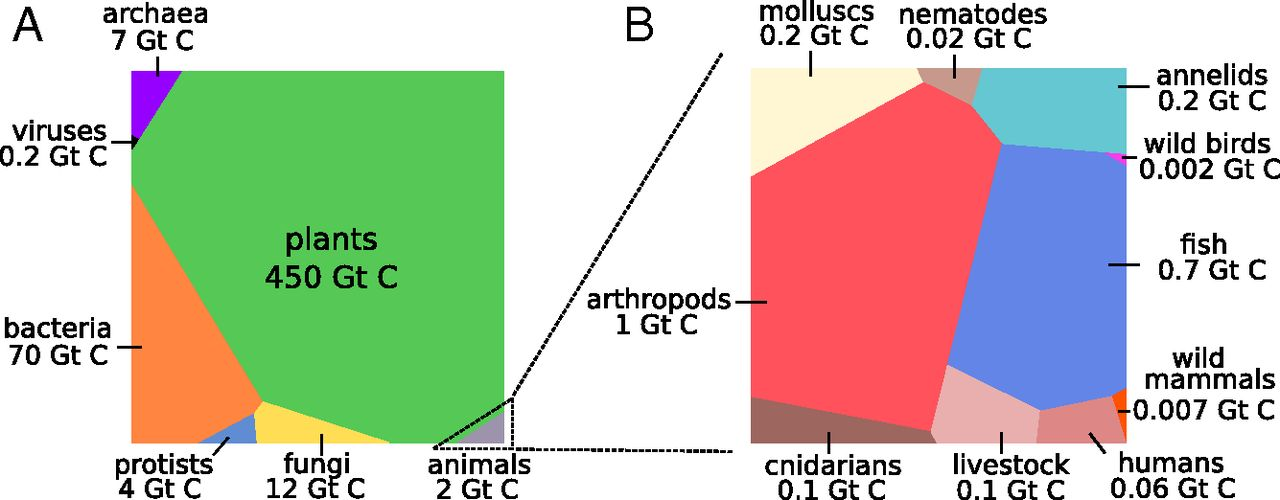
\includegraphics{figs/molbiol/biomass.jpeg}
  \caption[][6pt]{Distribution of biomass by taxa. Plants make up the majority of biomass on Earth, followed by bacteria and animals. Humans make up less than 1\% of the total biomass. The figure is from ``The biomass distribution on Earth'' by Bar-On, Phillips, and Milo (2018), published in the journal {\em Proceedings of the National Academy of Sciences} (PNAS), where they estimate the total biomass of Earth to be around 550 gigatons of carbon, with 80\% of this biomass composed of plants, 13\% of bacteria, and only 0.01\% attributed to humans. Most of the animal biomass is composed of arthropods and fish.}
  \label{fig:biomass}
% https://en.wikipedia.org/wiki/Cellular_compartment
\end{figure}

Oh, did we mention taxa? We did. Like computer scientists, biologists like to organize things and classify things into groups and hierarchies. Taxonomy is the science of classifying living things into groups based on common characteristics. The basic unit of taxonomy is the species, which is a group of organisms that can interbreed and produce fertile offspring. Species are further grouped into genera, families, orders, classes, phyla, and kingdoms. The highest level of classification is the domain, which is based on molecular data and includes three groups: Bacteria, Archaea, and Eukarya. These domains are based on differences in the genetic material of organisms and reflect the evolutionary relationships between them.

\begin{figure}
  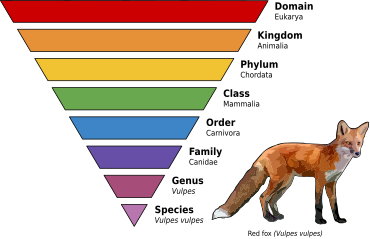
\includegraphics[width=0.8\textwidth]{figs/molbiol/taxonomy.png}
  \caption[][6pt]{Major ranks in biological taxonomy: from species at the bottom to domains at the top. Also shown is the naming of the red fox, \textit{Vulpes vulpes}. All living organisms are named according to their genus and species, and since these names are in Latin, they are italicised. The first letter of the genus is capitalised and the species name is lower case. Often biologists would shorten this naming by using the first letter of the genus and the full species name, as in the example of the red fox, \textit{V. vulpes}.}
  \label{fig:taxonomy}
% https://en.wikipedia.org/wiki/Cellular_compartment
\end{figure}


\section{Properties of Life}

Let's start by considering what defines something as living. Today we know that there are many types of organisms, including animals, plants, fungi, and microorganisms. Despite their differences, all living organisms share certain characteristics not found in non-living things. These characteristics of life include being composed of cells - the basic units of life - the ability to grow and develop, to reproduce, to respond to stimuli, and to maintain internal balance, like humans who maintain their body temperature at \(37^\circ\mathrm{C}\)). All of these functions require energy, which living organisms obtain by consuming food or other organisms. The ability to evolve and adapt to changing environments is another key characteristic of life. This is why we have so many different species on Earth, each adapted to its own niche.

\section{The Cell}

Cells are the Basic Units of Life
\marginnote{The number of cells in the human body comes from the study ``An estimation of the number of cells in the human body'' published by Bianconi et al. in the {\em Annals of Human Biology} (2013), which provides a comprehensive calculation of the number of cells in different tissues. The number is approximate, as it can vary depending on individual factors such as size and health.}
All living organisms consist of one or more cells. Cells are the building blocks of life and are responsible for carrying out the processes that sustain life. They are highly organized structures that contain all the necessary components to carry out the functions of life. 

Some organisms consist of a single cell, and we refer to them as single-celled organisms. Examples of single-celled organisms include bacteria, archaea, and protists. These organisms are capable of performing all the functions of life within a single cell. Single-celled organisms are the most abundant form of life on Earth and are found in almost every environment, from the deep sea to the soil to the human gut. They are of particular interest to biologists because a single cell can be easier to study than a complex organism with many cells. 

Single-celled organisms are classified as either prokaryotes or eukaryotes. Prokaryotes are single-celled organisms that lack a defined nucleus or other membrane-bound organelles. They include bacteria and archaea. Eukaryotes are single-celled organisms that have a defined nucleus and membrane-bound organelles. Examples of unicellular eukaryotes include certain types of algae, protozoa, and fungi such as yeast. (More on the nucleus later.)

Multicellular organisms are made up of many cells that work together. Humans, for example, are made up of \(6 \times 10^{13}\) cells. That's 60 trillion cells, or
$$ 60,000,000,000,000,000 {\ \rm cells}. $$
For comparison, there are about 300 billion stars in the Milky Way, so we have about 200 times more cells in our bodies than there are stars.

Molecular biologists used to define cell types based on how they looked under the microscope, but now we can also define them based on their molecular characteristics, such as the genes they express. There is a special field of molecular biology called single-cell transcriptomics, which studies the gene expression of individual cells. This field has revolutionized our understanding of cell types and their functions. More about this later in the course.

Figure~\ref{fig:cell} shows a diagram of a typical eukaryotic cell. Is it an animal or plant cell? What organelles can you identify? The cell is a complex structure with many different parts, each with a specific function. Some of the most important organelles in a eukaryotic cell are the nucleus, which contains the genetic material, the mitochondria, which produce energy, and the endoplasmic reticulum, which is involved in protein synthesis. Plant cells have some additional organelles, such as chloroplasts, which are involved in photosynthesis, and a large central vacuole, which stores water and nutrients.

\begin{figure}[h!]
    \centering{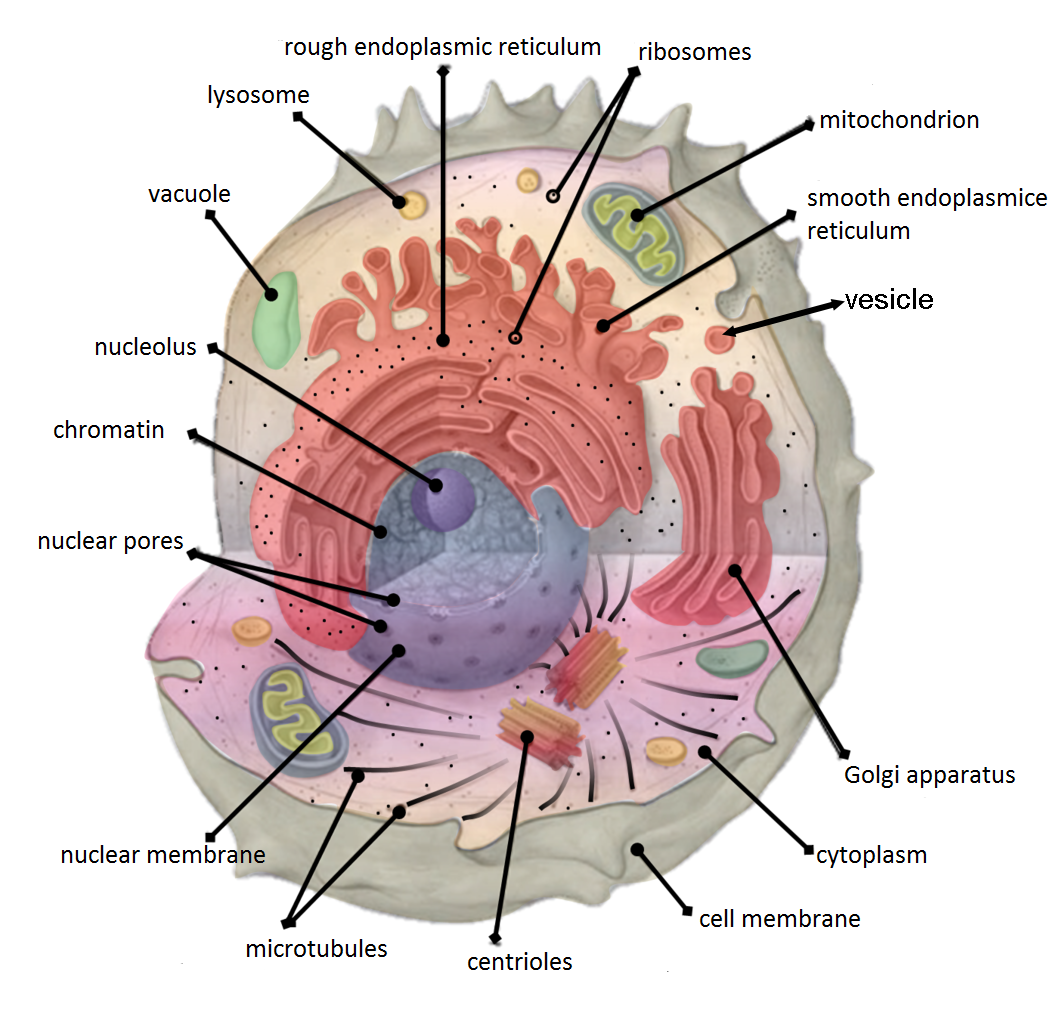
\includegraphics[width=0.8\textwidth]{figs/molbiol/cell.png}}
    \caption[][6pt]{The model of a eukaryotic cell, with some of its organelles labeled. Note that this is only a model, and that the actual cell is much more complex.}
    \label{fig:cell}
% https://en.wikipedia.org/wiki/Cellular_compartment
\end{figure}

\section{Cells Die and Are Replaced}

Cells in the human body are constantly dying and being replaced. Approximately 96 million cells die every minute as part of the natural process of cell turnover. The lifespan of a cell varies greatly depending on its type. For example, white blood cells typically survive for about 13 days, while epidermal skin cells last about a month. Red blood cells, which carry oxygen, have a lifespan of about 120 days. Liver cells, which are involved in vital metabolic processes, can live for about a year and a half before they are replaced. This continuous cycle of cell death and regeneration is essential for maintaining the health and function of the body.


\section{What Makes Up the Cell?}

A cell is made up of many components, but primarily water (about 70\%) and proteins (about 20\%). Water serves as the cell's medium, providing an environment in which biochemical reactions can take place. Proteins are large biomolecules, typically made up of thousands or more atoms, that play critical roles in the cell, acting as building blocks, catalyzing chemical reactions, and forming membranes.

The remaining 10\% of the cell is made up of smaller molecules, including sugars, fatty acids, signaling molecules, and energy-related molecules. If these smaller molecules were left alone, nothing significant would happen. It is the proteins that drive all essential cellular processes. They are the true engines of the cell, making everything that happens inside the cell happen, and ultimately sustaining life.

\section{Proteins}

Proteins are large, complex molecules that are essential to life. Proteins are involved in almost every process in the cell, from building and repairing tissues to regulating metabolism and transmitting signals. They are the workhorses of the cell, carrying out the functions that sustain life.

Proteins are made up of long chains of amino acids linked together in a specific sequence. All organisms, with a few exceptions, use 20 different amino acids that can be combined in different ways to make different proteins. The sequence of amino acids in a protein determines its structure and function. Proteins can have as few as 50 amino acids or as many as 30,000 amino acids. The average protein in a human cell contains approximately 300 amino acids.

Proteins have a complex three-dimensional structure that is critical to their function. A protein's structure is determined by its amino acid sequence and the interactions between the amino acids. Proteins can fold into specific shapes that allow them to interact with other molecules in the cell. The structure of a protein can be described on four levels: primary, secondary, tertiary, and quaternary. Primary structure refers to the sequence of amino acids in the protein. Secondary structure refers to the local folding of the protein chain into helices or sheets. The tertiary structure is the overall three-dimensional shape of the protein. The quaternary structure is the arrangement of several protein subunits into a larger protein complex.

For example, human insulin consists of 51 amino acids. The image in Fig.~\ref{fig:insulin-secondary} shows the secondary structure of human insulin. The secondary structure of a protein is (only) a sequence of amino acids that make up the molecule. In this figure, the amino acids are marked with circles containing a three-letter abbreviation. For example, the insulin chain begins with Met, which is an abbreviation for methionine. The secondary structure of a protein is important because it determines how the protein will fold into its three-dimensional shape.

\begin{figure}
    \centering{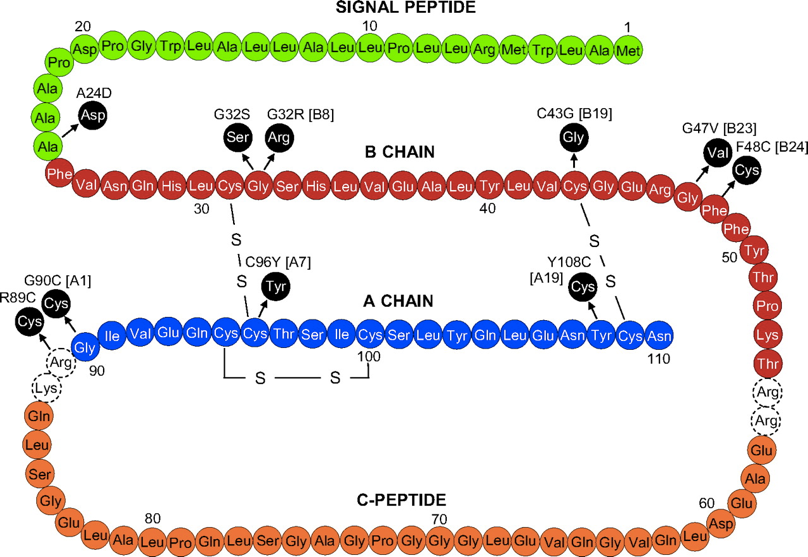
\includegraphics[width=0.9\textwidth]{figs/molbiol/insulin-chain.png}}
    \caption[][6pt]{Secondary structure of insulin.}
    \label{fig:insulin-secondary}
\end{figure}

The folding of a protein defines its function. Its tertiary structure gives the actual three-dimensional structure of the protein. Fig.~\ref{fig:insulin-3d} is what insulin looks like in 3D, where the representation of the amino acid sequences has been abstracted with parts that look like sheets and helices (don't worry about them now).

\begin{figure}
    \centering{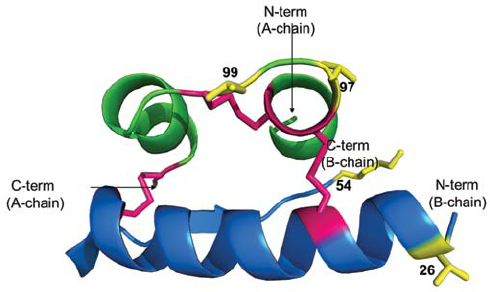
\includegraphics[width=0.7\textwidth]{figs/molbiol/insulin-3d.png}}
    \caption[][6pt]{Tertiary structure of an insulin.}
    \label{fig:insulin-3d}
\end{figure}

A protein's structure is critical to its function. Proteins can fold into complex three-dimensional shapes that allow them to interact with other molecules in the cell. The shape of a protein is determined by its amino acid sequence and the interactions between the amino acids. Proteins can also change shape in response to signals from the cell to perform specific functions.

Another example: a leptin (Figure~\ref{fig:leptin}). Leptin is a hormone that helps regulate energy balance by inhibiting hunger. It is composed of 167 amino acids, and its tertiary structure is shown below. Leptin deficiency leads to obesity. Molecular biologists have studied this in several model organisms, including mice.

\begin{figure}
    \centering{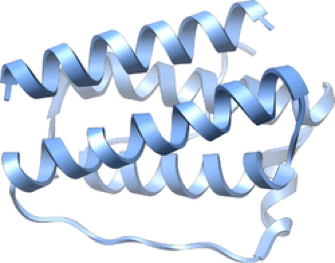
\includegraphics[width=0.6\textwidth]{figs/molbiol/leptin.png}}
    \caption[][6pt]{Tertiary structure of a leptin.}
    \label{fig:leptin}
\end{figure}

The three-dimensional structures of proteins are often quite amazing. Consider chaperonins, a class of proteins that provide favorable conditions for the proper folding of other proteins. Fig.~\ref{fig:chaperonin} shows a rendering of what they look like. Chaperonins form a protective chamber that allows proteins to fold correctly without interference from other molecules. Chaperonins are found in all cells and are critical for maintaining the health and function of the cell.
    
\begin{figure}
    \centering{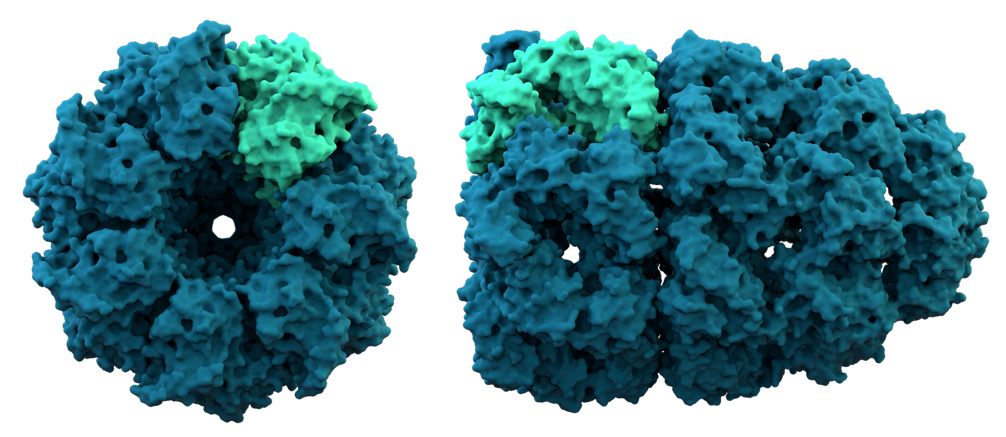
\includegraphics[width=0.8\textwidth]{figs/molbiol/chaperonin.png}}
    \caption[][6pt]{Tertiary structure of a chaperonin.}
    \label{fig:chaperonin}
\end{figure}

\section{Amino Acids}

We have talked about amino acid chains, but we have never really said what they are. Now is the time. An amino acid is a simple organic compound containing both a carboxylic acid (-COOH) and an amino group (-NH2). Plus a side chain (labeled R). Fig.~\ref{fig:aminoacid} is their chemical structure.

\begin{marginfigure}
    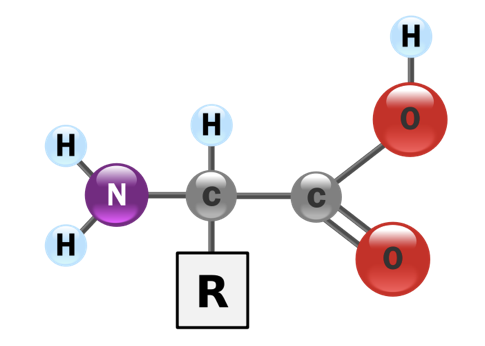
\includegraphics{figs/molbiol/aminoacid.png}
    \caption[6pt]{Chemical structure of an amino acid.}
    \label{fig:aminoacid}
\end{marginfigure}

The side chain is what defines each amino acid. Around 500 amino acids are known, but only twenty commonly appear in living organisms. It's worth noting that there are exceptions, as biology often defies strict rules, but this isn't the time to dive into those details. Some side chains are very simple; for example, the side chain of glycine is just a single hydrogen atom. Fig.~\ref{fig:aminoacids} shows all twenty side chains and the corresponding names of their amino acids.

\begin{figure}
    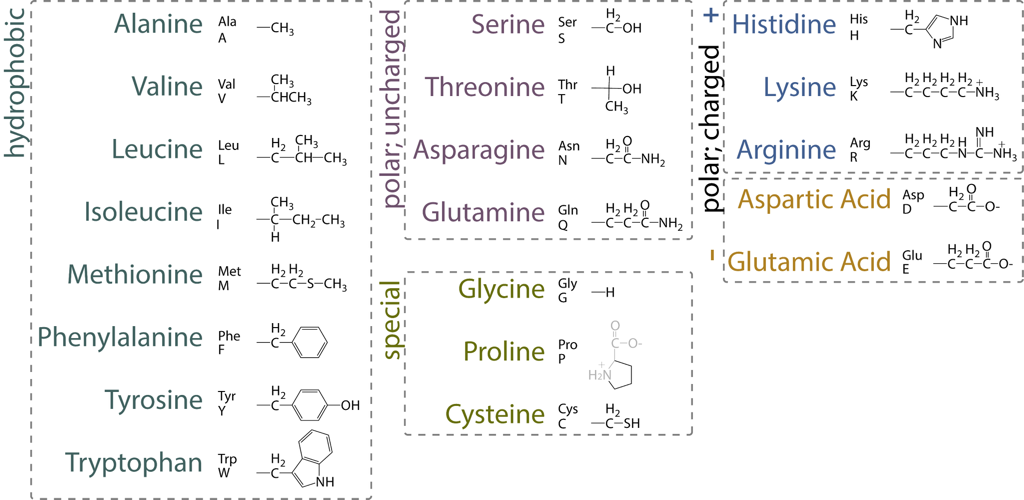
\includegraphics{figs/molbiol/aminoacids.png}
    \caption[6pt]{Chemical structure of an amino acid.}
    \label{fig:aminoacids}
\end{figure}

Proteins are chains of amino acids. They are actually made by stitching amino acids together, in a row, one by one. The process is called polymerization, a condensation reaction where two amino acids are stitched together via a peptide bond between nitrogen and carbon. Here is a graphical depiction of the process. Fig.~\ref{fig:peptide-bond} shows the reaction that forms a peptide bond between two amino acids. The amino acids are shown in their abbreviated form, with the side chain represented by the letter R. The peptide bond is formed between the carboxyl group of one amino acid and the amino group of the other amino acid. The resulting molecule is called a dipeptide.

\begin{figure}
    \centering{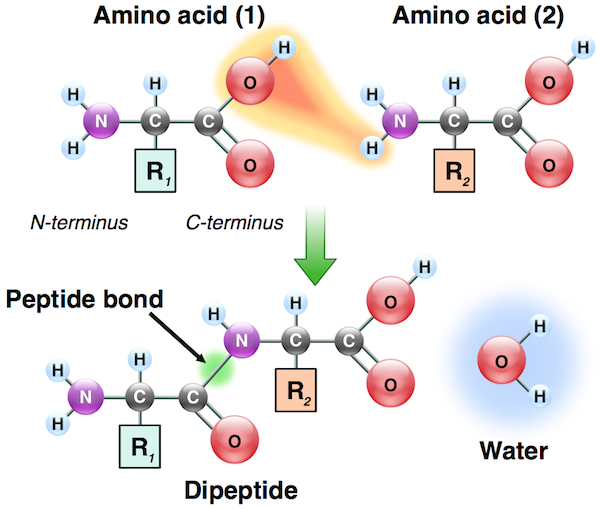
\includegraphics[width=0.65\textwidth]{figs/molbiol/peptide-bond.png}}
    \caption[6pt]{Formation of a peptide bond between two amino acids.}
    \label{fig:peptide-bond}
\end{figure}

The process of polymerization continues until the protein is complete. The resulting chain of amino acids is called a polypeptide. The polypeptide chain can then fold into a specific three-dimensional shape that determines the protein's function. The folding of a protein is a complex process that is influenced by many factors, including the amino acid sequence, the environment of the cell, and the interactions between the amino acids.

\section{Metabolism}

Metabolism is the set of chemical reactions that occur in living organisms to maintain life. These reactions are essential for the growth, development, and reproduction of organisms. Metabolism can be divided into two main categories: catabolism and anabolism. Catabolism refers to the breakdown of complex molecules into simpler ones, releasing energy in the process. Anabolism refers to the synthesis of complex molecules from simpler ones, requiring energy. Together, catabolism and anabolism maintain the balance of energy in the cell and allow the cell to carry out its functions.

Metabolism is regulated by enzymes, which are proteins that catalyze chemical reactions in the cell. Enzymes are highly specific and only catalyze specific reactions. They can speed up reactions by a factor of up to a billion times. 

Here is an example of a metabolic pathway: glycolysis. Glycolysis is the breakdown of glucose into pyruvate, a process that releases energy. The process of glycolysis is shown in Fig.~\ref{fig:glycolysis}. Glycolysis is the first step in cellular respiration, a process that generates energy for the cell. The energy released during glycolysis is used to produce ATP, the cell's primary energy source.

\begin{figure*}
    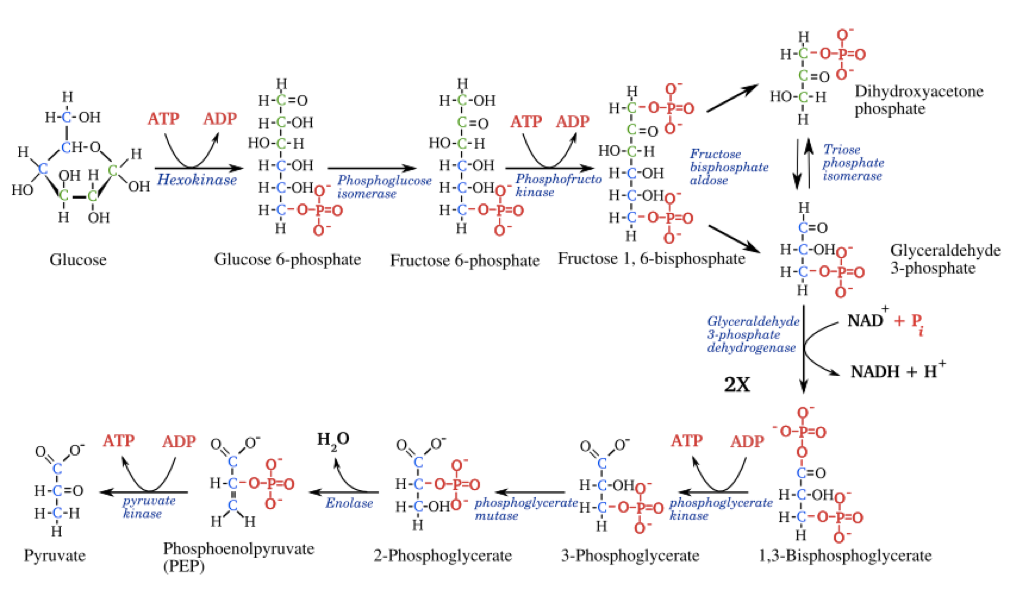
\includegraphics{figs/molbiol/glycolysis.png}
    \caption[6pt]{The glycolysis pathway.}
    \label{fig:glycolysis}
\end{figure*}

Chemicals such as glucose, fructose 6-phosphate, and others that serve as entry points, final products, or intermediates in chemical reactions are called metabolites. Glycolysis is an example of a metabolic pathway. All the reactions in glycolysis are catalyzed by enzymes, which are proteins that drive reactions that wouldn't occur on their own. Proteins in this and other pathways often have complex names that are difficult for computer scientists to remember :). For example, the enzyme that converts glucose 6-phosphate to fructose 6-phosphate is called phosphofructokinase. Fortunately, we don't need to memorize these names, but it's crucial to understand that almost no reaction in living organisms would happen without proteins. Proteins are essential to metabolic pathways and are key to making cells function and stay alive. 

Just for a taste, Fig~\ref{fig:glycolysis} is how hexokinase looks like (find it in glycosylation pathway, what does it do?). It consists of 617 aminoacids.

\begin{figure}
    \centering{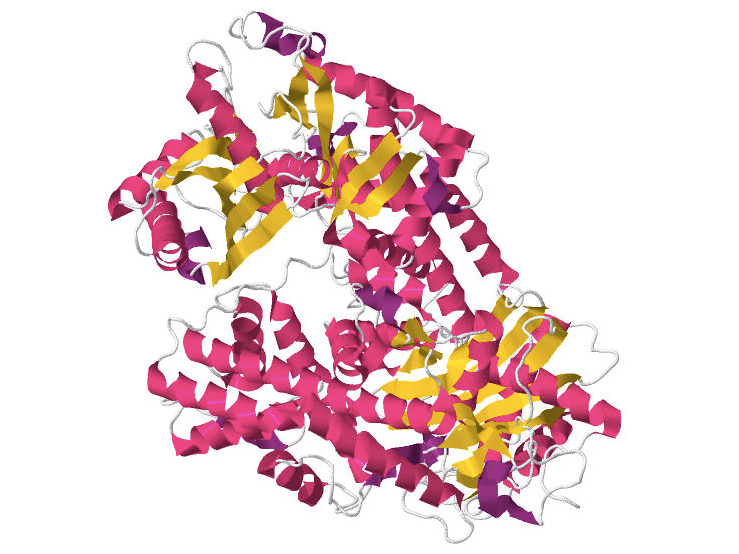
\includegraphics[width=0.7\textwidth]{figs/molbiol/hexokinase.png}}
    \caption[][6pt]{Tertiary structure of a hexokinase.}
    \label{fig:hexokinase}
\end{figure}

\section{Some More Surprising Facts}

A typical protein is about 5 nm in size, while a typical eukaryotic cell is around 500 µm. The diameter of a cell is approximately 10,000 times larger than that of an average protein. Since volume scales with the cube of the diameter, the volume of the cell is roughly $10,000^3 = 10^{12}$ times larger than the volume of a typical protein.

Incredibly, each cell contains about one billion protein molecules, or $1,000,000,000$ molecules. Wow!

To add more perspective, there are about two million different proteins in the human body. The longest known protein is a chain of 27,000 amino acids!

\section{Proteins Degrade}

Ok, so we have quite many proteins in each cell. They are there, do some work, and stay there and nothing changes. This is nicely supported by the biology we have learned in the high school where it was said that the enzymes are not wasted in the reactions. So, the enzymes and the rest of the protein are just there forever. Right?

Wrong. The proteins have their lifespan. They do not last forever. They degrade. In a matter of hours. Here's the abstract of the publication where they have measured degradation rates (half-lives) for rat enzymes\marginnote{The publication is ``Degradation of glucose-metabolizing enzymes in the rat small intestine during starvation'' by G M Jones and R J Mayer, published in the {\em Biochemical Journal} (1973).}:

\begin{quote}
    \textit{1. The degradation rates and half-lives of hexokinase, 6-phosphogluconate dehydrogenase, lactate dehydrogenase, pyruvate kinase, glucose 6-phosphate dehydrogenase, phosphoglycerate kinase and aldolase were calculated from measurements of the decline in activities of these enzymes in rat small intestine during starvation. 2. The half-lives of the enzymes are: hexokinase, 5.7h; 6-phosphogluconate dehydrogenase, 7.6h; glucose 6-phosphate dehydrogenase, 6.0h; pyruvate kinase, 8.9h; lactate dehydrogenase, 8.7h; phosphoglycerate kinase, 8.7h; aldolase, 5.1h. 3. The significance of the results is discussed with respect to the regulation of enzyme concentrations in response to changes in diet.}
\end{quote}

\section{The Puzzle}

So now we know that there are lots of proteins in cells. And proteins are what keep us alive. But they do not last very long. Someone has to make them. But who? Where? Is there a factory for each of the two million different proteins? Or is there a single factory that makes the proteins according to a given recipe? But where is the recipe?

\section{The Central Dogma of Molecular Biology}

The central dogma of molecular biology is a framework that describes the flow of genetic information in cells. It states that genetic information flows from DNA to RNA to protein. This information flow is unidirectional and irreversible. The central dogma is a fundamental principle of molecular biology and is essential for understanding how genetic information is stored, replicated, and expressed in living organisms.

In a nutshell, as it took scientists ages and numerous Nobel Prizes to figure out, the recipes for all the proteins involved in our lives are stored in a long molecule called DNA (Fig.~\ref{fig:dna-detail}), or deoxyribonucleic acid. In eukaryotes, DNA is tightly packed and stored in the nucleus of the cell. DNA is in the form of a double helix, with two complementary strands. Each strand is a chain of nucleotides attached to a sugar backbone that is linked together by phosphate bonds.

\begin{figure}
    \centering{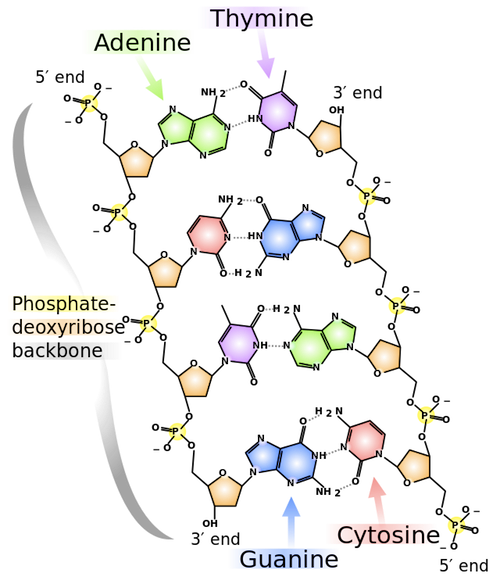
\includegraphics[width=0.7\textwidth]{figs/molbiol/dna-detail.png}}
    \caption[6pt]{The structure of DNA.}
    \label{fig:dna-detail}
\end{figure}

There are only four different nucleotides, cytosine (C), guanine (G), adenine (A), or thymine (T). Across the strands, thymine can make hydrogen bound with adenine, and cytosine with guanine (Fig.~\ref{fig:tacg-bonds}). The strands are therefore complementary and carry, at least when considering only the sequence of the nucleotides, identical information.

\begin{figure}
    \centering{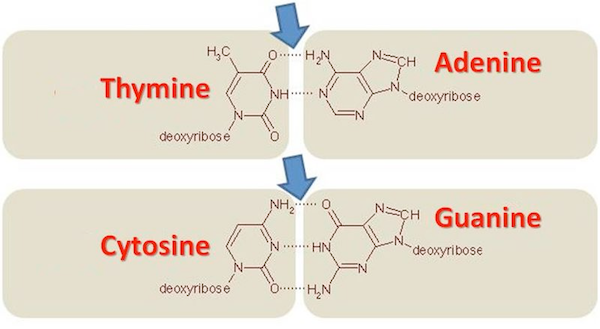
\includegraphics[width=0.8\textwidth]{figs/molbiol/tacg-bonds.png}}
    \caption[6pt]{Hydrogen bonds between nucleotides in DNA.}
    \label{fig:tacg-bonds}
\end{figure}

Did we say information? So soon! We were not there yet. But let us hurry (Fig.~\ref{fig:central-dogma}): Proteins are made in the cytoplasm, in factories called ribosomes. DNA, or rather a small subsequence of DNA, which, as part of its chain, has a recipe for the protein. This recipe must first come from the nucleus and then arrive at the ribosome. The carrier molecule is called RNA, a ribonucleic acid. To conserve energy and not make too much mess, Mother Nature figured out that it would be best to copy only the part of the DNA that encodes the amino acid sequence that makes up the protein onto the RNA. This copying process is called transcription. The RNA (called messenger RNA because of its function) then travels from the nucleus to the ribosome, where the sequence of amino acids is translated into a sequence of proteins.

\begin{figure}
    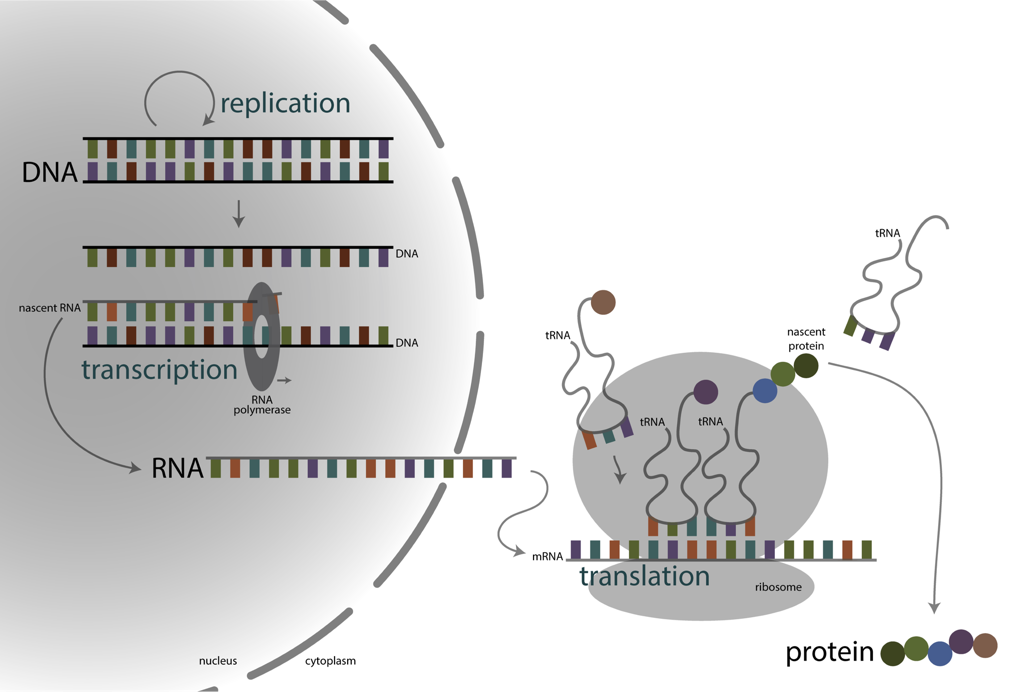
\includegraphics{figs/molbiol/central-dogma.png}
    \caption[][6pt]{The central dogma of molecular biology.}
    \label{fig:central-dogma}
\end{figure}

There are twenty amino acids that we need to encode. Encoding language consists of an alphabet of four nucleotides. One letter of an alphabet is not sufficient to represent one of twenty amino acids. We need words. Say that the length of the word is constant (we admit here that this is weird, but it is the most simple solution so in the light of Occam's razor this assumption is perfectly ok). Such words. If we had words made of two nucleotides, they would encode for $4\times 4$ different amino acids. Not enough, we have twenty to provide encoding for. So we need at least three-letter words or a sequence of three nucleotides. And, through evolution, a language with three-letter words emerged, each word encoding for one of the amino acids. Different words are encoding for the same amino acid, as there are $4\times 4\times 4=64$ different combinations with a sequence of three nucleotides.

\begin{figure}
    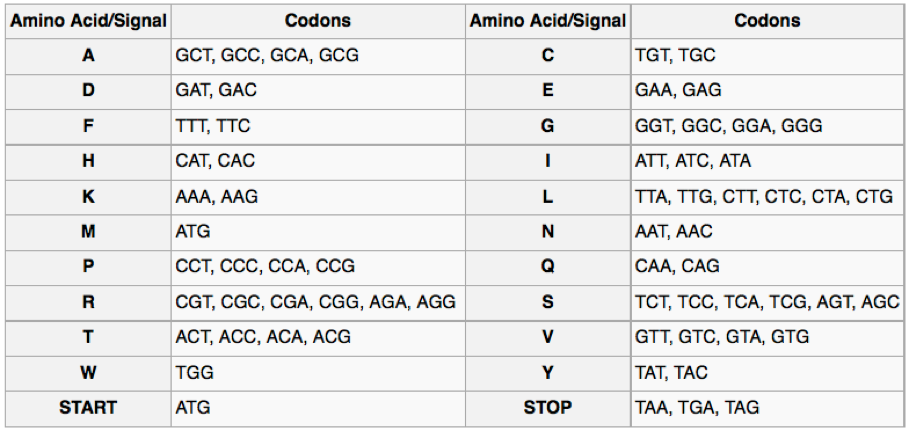
\includegraphics{figs/molbiol/code-of-life.png}
    \caption[][6pt]{The genetic code.}
    \label{fig:code-of-life}
\end{figure}

The sequence of three nucleotides is called a codon. The codon is the basic unit of the genetic code. The genetic code is the set of rules that determines how the nucleotide sequence of a gene is translated into the amino acid sequence of a protein. The genetic code is universal, meaning that the same codons encode the same amino acids in all living organisms. The genetic code is redundant, meaning that most amino acids are encoded by more than one codon. The genetic code is also non-overlapping, meaning that each nucleotide is part of only one codon.

\section{What's Next?}

This is the beginning of molecular biology. But there are tons of open questions at this point. Here are just a few. For example, where are the parts of the DNA that contain the coding information for the proteins? How does transcription know where to find them? How many are there in all of DNA? How long is DNA, how many nucleotides are there? Is there any other information stored in DNA? Are all proteins being made all the time? If not, by whom and how is this process regulated? Enough for this chapter. We should leave something for the rest of the course.